%!TeX root = Chapter_Method
\documentclass[../../CompleteThesis/Complete_1stDraft.tex]{subfiles}
\begin{document}
This section contains a walk through of the method to back diffuse a given ice core depth series to attempt to restore as much of the original signal as possible. For now, the method has been developed for sections that has been dated to be between the two volcanic eruptions Laki and Tambora, as these are very well dated, and thus it is possible to find the optimal diffusion length to back diffuse with as the actual number of annual layers is exactly known for this data series. The method is easily modified for any other dated depth series, as what is needed is just the number of annual layers in the given data series.\\
Figure \ref{Fig:FlowchartDiffLen} shows a flowchart of the method used to estimate the diffusion length of a depth series with a preliminary guess of number of annual layers. In the following sections each of the steps in the method will be discussed more thoroughly and examples will be given, all based on the Greenlandic ice core drilled at Site A near Crete(REFERENCES!!!).
The method is built such that it takes two inputs - the isotopic depth series, and the specifications for the particular ice core - and uses these for the first preliminary computations needed to make a first, naïve guess of the diffusion length, $\sigma_0$.
This diffusion length is then used to deconvolute the data and give a first estimate of the number of peaks in the data series. If this number is different from the already specified number of annual layers - in this case 32 - then the diffusion length will be updated accordingly: If the counted number is higher(lower) than the actual number, the diffusion length is adjusted downwards(upwards) with $\Delta\sigma_2$ and the deconvolution and peak counting is performed again.
On the other hand, if the counted number is equal to the actual number, then the diffusion length is optimized to find the largest diffusion length which still gives the actual number of counted peaks. When this $\sigma_{\text{final}}$ is reached, the algorithm stops and returns the final diffusion length estimate along with the associated back diffused depth series.
\begin{figure}
	\begin{tikzpicture}[node distance=1.5cm, auto]
		\node(start) [startstop] {START};
		%----------------------------------------------------%
		\node(in1) [io, left of=start, xshift=-3.5cm] {Depth series};
		\node(in1pro1) [process, below of=in1, yshift=-0.5cm] {Spline interpolation};
		\node(in1pro2) [process, below of=in1pro1] {Spectral analysis};
		\node(in1pro3) [process, below of=in1pro2] {Wiener filter};
		%	\node(in1pro4) [process, below of=in1pro3] {\textbf{Frequency filters}};	
		
		\draw[arrow] (in1) -- (start);
		\draw[arrow] (start) |- (in1pro1);
		\draw[arrow] (in1pro1) -- (in1pro2);
		\draw[arrow] (in1pro2) -- (in1pro3);
		%	\draw[arrow] (in1pro3) -- (in1pro4);
		
		%----------------------------------------------------%
		\node(in2) [io, right of=start, xshift=3.5cm] {Core specs};
		\node(in2pro1) [process, below of=in2, yshift=-0.5cm] {Density profile};
		\node(in2pro2) [process, below of=in2pro1] {Diffusion profile};
		\node(in2pro3) [process, below of=in2pro2] {$\sigma_0$\textbf{ estimate}};
		
		\draw[arrow] (in2) -- (start);
		\draw[arrow] (start) |- (in2pro1);
		\draw[arrow] (in2pro1) -- (in2pro2);
		\draw[arrow] (in2pro2) -- (in2pro3);
		
		%----------------------------------------------------%
		\node(pro0) [process, below of=start, yshift=-4.5cm] {\textbf{Frequency Filters}};
		\node(pro1) [process, below of=pro0] {\large{\textbf{BACK DIFFUSE}}};
		\node(pro2) [process, below of=pro1] {Count N Peaks};
		\node(dec1) [decision, below of=pro2, yshift=-.5cm] {$N = 32$ ? };
		
		\draw[arrow] (in1pro3) -| (pro0);
		\draw[arrow] (in2pro3) -| (pro0);
		\draw[arrow] (pro0) -- (pro1);
		\draw[arrow] (pro1) -- (pro2);
		\draw[arrow] (pro2) -- (dec1);
		
		%----------------------------------------------------%	
		\node(pro3a) [process, below of=dec1, xshift=-3cm] {$\sigma = \sigma + \Delta \sigma_1 $};
		\node(pro3apro1) [process, below of=pro3a] {Back diffuse};
		\node(pro3apro2) [process, below of=pro3apro1]  {Count N peaks};
		\node(pro3apro3) [process, below of=pro3apro2, xshift=-2cm] {$\sigma_{\text{final}} = \sigma - 2\cdot\Delta\sigma_1$};
		\node(stop) [startstop, right of=pro3apro3, xshift=2.5cm] {STOP};
		\node(out1) [io, right of=stop, xshift=2.5cm, text width=2.5cm] {\footnotesize{back diffused depth series}};
		\node(out2) [io, below of=out1, text width=1.1cm] {$\sigma_{\text{final}}$};
		
		
		\draw [arrow] (dec1) -| node[anchor=east] {yes} (pro3a);
		\draw [arrow] (pro3a) -- (pro3apro1);
		\draw [arrow] (pro3apro1) -- (pro3apro2);
		\draw [arrow] (pro3apro2) --++ (2,0) node [anchor=west] {If $N$ = 32} |- (pro3a);		
		\draw[arrow] (pro3apro2) --++ (-2,0) node [anchor=east] {If $N > $  32} -| (pro3apro3);
		\draw[arrow] (pro3apro3) -- (stop);
		\draw[arrow] (stop) -- (out1);
		\draw[arrow] (stop) |- (out2);
		
		%----------------------------------------------------%	
		\node(pro3b1) [process, right of=dec1, xshift=3.2cm] {$\sigma = \sigma - \Delta\sigma_2$};
		\node(pro3b2) [process, below of=dec1, xshift=4.7cm] {$\sigma=\sigma+\Delta\sigma_2$};
		
		
		\draw [arrow] (dec1) --(2.45,-11) node[anchor=south] {$N > 32$} -- (pro3b1);
		\draw[arrow] (dec1) -- (0,-12.5) node[anchor=north] {$N < 32$} -- (pro3b2);
		\draw[arrow] (pro3b1) |- (pro1);
		\draw [arrow] (pro3b2) --++ (2,0) |- (pro1);		
		
	\end{tikzpicture}
	\caption[Flowchart]{Flowchart of method for diffusion length computation.}
	\label{Fig:FlowchartDiffLen}
\end{figure}	




\subsection[Input]{Input}
To compute the final diffusion length and depth series, two inputs are needed: the measured isotopic depth series and the specifications of the examined core. Through this section all examples have been carried out using the core Site A.\\
\begin{figure}
	\centering
	\includegraphics[width=0.9\textwidth]{SiteA_d18OInsert.jpg}
	\caption[Full $\delta^{18}$O record with insert, Site A]{The entire ice core isotopic profile from Site A, with a zoom in on the estimated depth series spanning from Tambora to Laki.}
	\label{fig:SiteA_d18OInsert}
\end{figure}

CORE SPECIFICATIONS TABLE 
Along with coordinates, height above sea, etc.



In Figure \ref{fig:SiteA_d18OInsert} the depth series between the eruptions Laki and Tambora can be seen along with the entire ice core in the background. This is the diffused, measured raw data from Site A. Dating of the ice cores has been carried out by matching Electrical Conductivity Measurements (ECM, Section \ref{Sec:??}) with water isotopic - in this case $\delta^{18}$O - data measured at the same depths. By doing so it is possible to identify known volcanic horizons in the ECM data and thus getting a sharp marker of when the precipitation of that given depth fell. In Figure \ref{fig:SiteA_ECMd18O_combo} the matched ECM and $\delta^{18}$O profiles can be seen with Tambora marked at depth \_\_\_\_ and Laki at depth \_\_\_\_.



\begin{figure}[h]
	\centering
	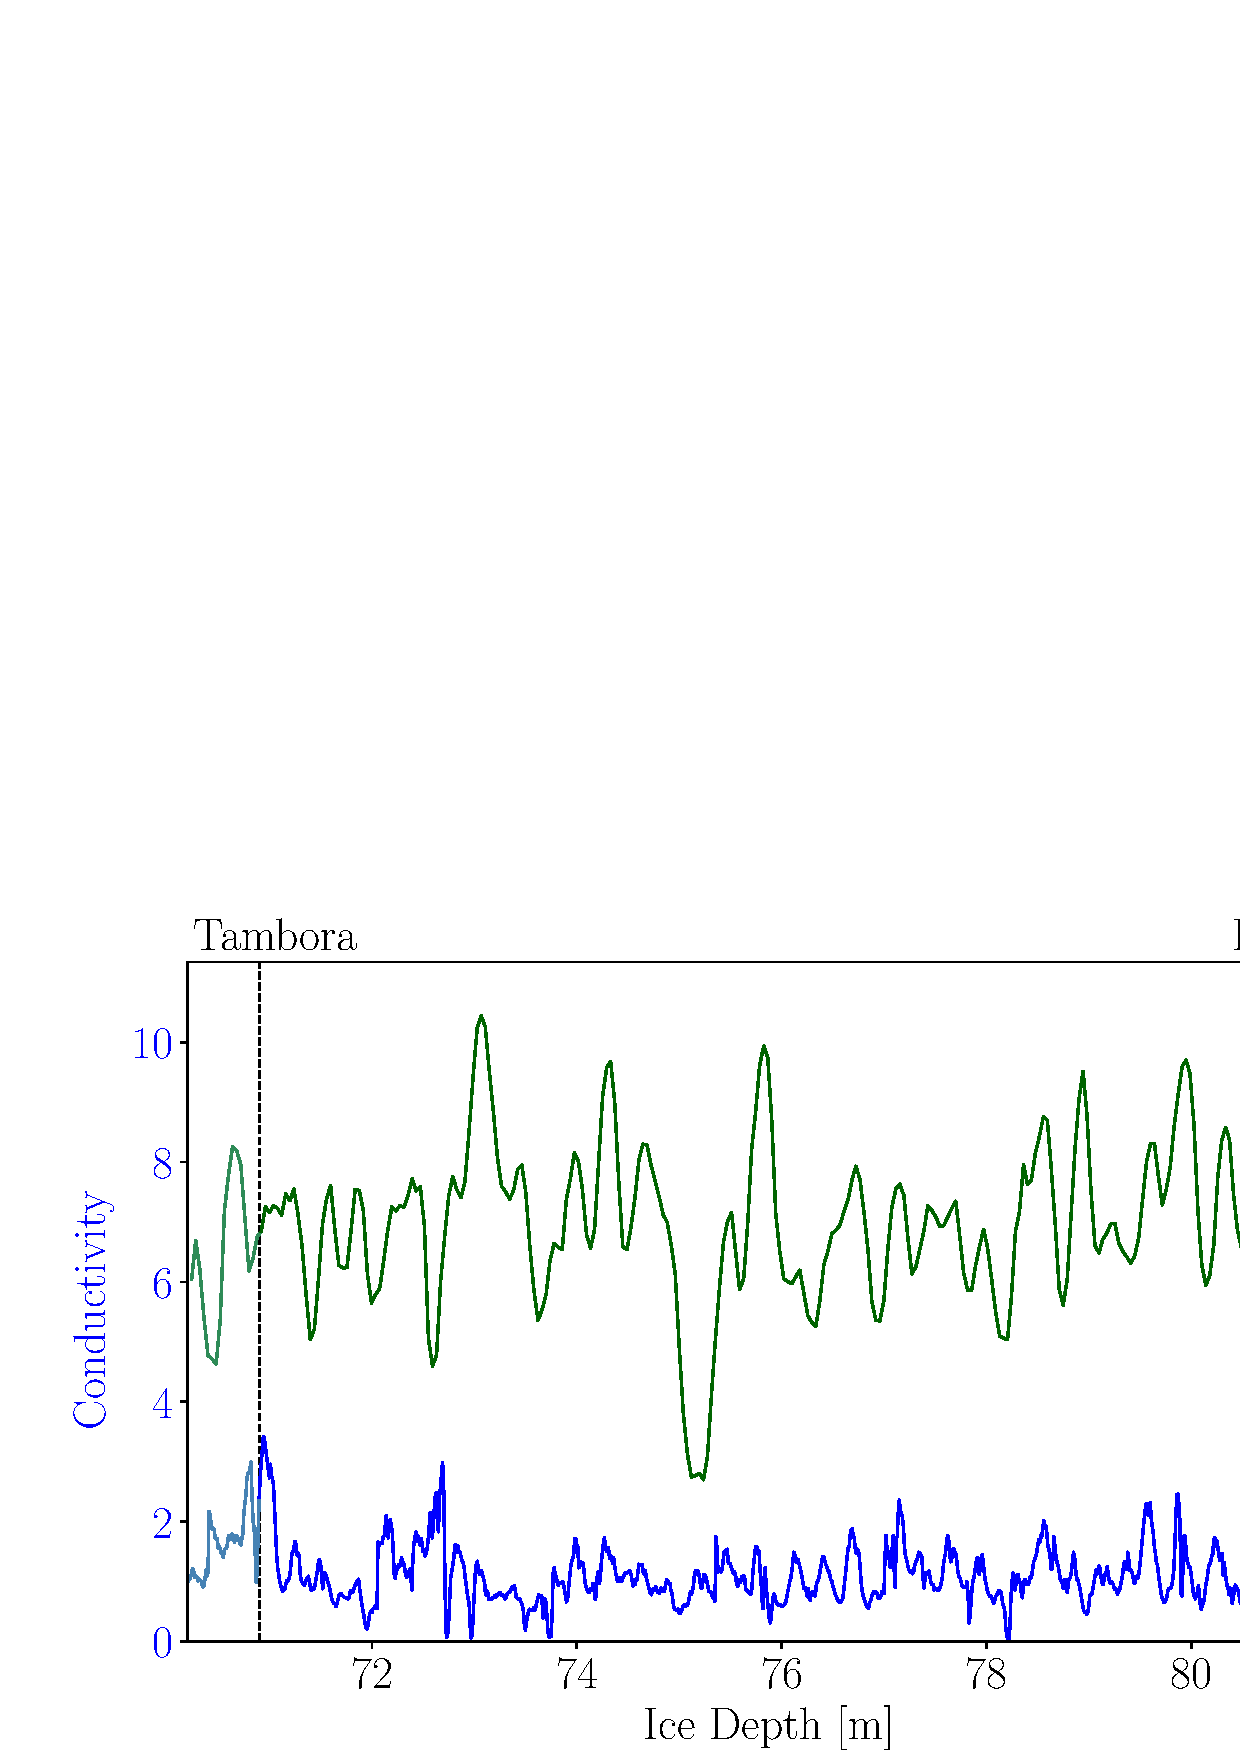
\includegraphics[width=0.9\textwidth]{SiteA_ECMd18O_combo.jpg}
	\caption[ECM and d18O data at LT, Site A.]{Two depth profiles from the core drilled at Site A showing accordingly the measured $\delta^{18}$O isotopic values and the conductivity measurements in the depth ranging from the estimated Tambora eruption to the Laki eruption.}	
	\label{fig:SiteA_ECMd18O_combo}
\end{figure}

\subsection[Preliminary Computations]{Preliminary Computations}
From the inputs a number of preliminary computations need to be carried out before the optimization of the diffusion length can be performed. For the depth series this consists of first interolating the data to make sure that the depth series is evenly sampled, then an analysis of signal and noise in the frequency spectrum needs to be carried out, and from this spectral analysis a Wiener filter can be constructed to find the optimal high frequency cut off, where as much noise as possible is filtered away while losing as little of the signal as possible. These computations are all based on the depth series data and use only signal analysis theory.\\
The input of core specifications on the other hand is used to give a more theoretical view of the situation. From these preliminary inputs, containing accumulation rate, borehole temperatures, altitudes and other conditions, it is possible to use ice core and ice flow theory to compute initial estimates of density and diffusion profiles at the given site. From these profiles along with the volcanic horizons indicating the series of interest, an initial estimate of the diffusion length at the depth of Laki to Tambora.
 
\subsubsection[Spline Interpolation]{Depth Series: Spline Interpolation}
\begin{figure}[h]
	\centering
	\includegraphics[width=0.9\textwidth]{SiteA_d18OLT_Interp.jpg}
	\caption[Measured and interpolated $\delta^{18}$O data, Site A]{The unevenly measured data from Site A in the depth ranging from Tambora to Laki along with the now evenly sampled cubic spline interpolated data. Sampled with an interval of $\Delta = 0.038$.}
	\label{fig:SiteA_d18OLT_Interp}
\end{figure}

\subsubsection[Spectral Analysis]{Depth Series: Spectral Analysis}
\begin{marginfigure}
	\centering
	\begin{subfigure}{\marginparwidth}
		\centering
		\includegraphics[width=\textwidth]{SiteA_PSD_sig.jpg}
		\caption{\footnotesize{Signal estimate given through fitting to all data (noise and signal).}}
		\label{fig:SiteA_PSD_sig}
	\end{subfigure}\\[1ex]
	
	\begin{subfigure}{\marginparwidth}
		\centering
		\includegraphics[width=\textwidth]{SiteA_PSD_noise.jpg}
		\caption{\footnotesize{Noise estimate given through fitting to all data (noise and signal).}}
		\label{fig:SiteA_PSD_noise}
	\end{subfigure}\\[1ex]
	
	\begin{subfigure}{\marginparwidth}
		\centering
		\includegraphics[width=\textwidth]{SiteA_PSD_fit.jpg}
		\caption{\footnotesize{Complete spectral fit to all data (blue), both noise and signal.}}
		\label{fig:SiteA_PSD_fit}
	\end{subfigure}
	\caption[Isolated spectral fits, Site A]{Spectral fits.}
	\label{fig:SpectralFitsIsolated}
\end{marginfigure}




\begin{figure}[h]
	\centering
	\begin{subfigure}{.45\textwidth}
		\centering
		\includegraphics[width=\textwidth]{SiteA_DCT_PSD_raw.jpg}
		\caption[PSD of LT data, Site A]{The power spectral density(PSD) of the interpolated data from Site A shown in Figure \ref{fig:SiteA_d18OLT_Interp}. The PSD was computed through a Discrete Cosine Transform(DCT).}
		\label{fig:SiteA_DCT_PSD_raw}
	\end{subfigure}
	~
	\begin{subfigure}{0.45\textwidth}
		\includegraphics[width=\textwidth]{SiteA_PSD_all}
		\caption[Spectral fit, Site A]{Spectral estimate of the depth series from Tambora to Laki along with fit to entire spectral data set and the separated estimates of the noise and signal functions, as described in section \ref{sec:??}. }%Signal(blue), noise(green) and fit(black).}
		\label{fig:SpectralFitsAll}
	\end{subfigure}
\end{figure}

\subsubsection[Frequency Filters]{Depth Series: Frequency Filters}
\begin{figure}[h]
	\centering
	\includegraphics[width=\textwidth]{SiteA_filtersEx.jpg}
	\caption[Frequency filters example, Site A]{Frequency filter examples ranging from diffusion length 0.04 m to 0.085 m.}
	\label{fig:SiteA_filtersEx}
\end{figure}

\subsubsection[Density Profile]{Core Specifications: Density Profile}
\begin{marginfigure}
	\centering
	\includegraphics[width=\marginparwidth]{SiteA_DensProfile_wHL.jpg}
	\caption[Density profile Site A]{\footnotesize{Depth density profile at Site A. Black is the measured densities during drilling, blue is the modelled density profile given a Herron Langway model, and orange is a Herron Langway model with a criterion to minimize the distance to the actual measurements.}}
	\label{Fig:SiteA_DensProfile_wHL}
\end{marginfigure}


\subsubsection[Diffusion Profile]{Core Specifications: Diffusion Profile}
\begin{marginfigure}
	\centering
	\includegraphics[width=\marginparwidth]{SiteA_DiffProfile.jpg}
	\caption[Diffusion profile, Site A.]{\footnotesize{Estimated diffusion profile at Site A given a Herron Langway model.}}
	\label{fig:SiteADiffProfile}
\end{marginfigure}

\subsubsection[$\sigma_0$ estimate]{Core Specifications: $\sigma_0$ estimate}

\subsection[Back Diffusion]{Back Diffusion/Deconvolution}

\subsection[Peak Counting]{Peak Counting}

\subsection[Decision algorithm]{Decision Algorithm}

\subsection[Output]{Output}


\begin{figure}
	\centering
	\includegraphics[width=0.9\textwidth]{SiteA_BackDiffused_Y32.jpg}
	\caption[Best estimate of deconvoluted depth series, Site A]{Best estimate of deconvoluted depth series given an annual count of 32 years - marked as orange dots. The best estimate is taken as the largest diffusion length that still yields 32 years in the depth span from Tambora to Laki.}
	\label{fig:SiteA_BackDiffused_Y32}
\end{figure}

\begin{figure}
	\centering
	\includegraphics[width=\textwidth]{SiteA_BackDiffused_AllSigmaEst.jpg}
	\caption[All diffusion length estimate deconvolutions, Site A]{Estimated back diffused data series with different diffusion length estimates: diffusion length estimate from spectral fit ($\sigma_{fit}$), maximum ($\sigma_{Max}^{Theo}$) and minimum ($\sigma_{Min}^{Theo}$) theoretically estimated diffusion lengths and final estimated diffusion length.}
	\label{fig:SiteA_BackDiffused_AllSigmaEst}
\end{figure}















\end{document}
